\section{Estado del arte}

Como decíamos anteriormente, la investigación en visión artificial se ha convertido en sinónimo de deep learning, siendo uno de los dominios donde más progreso se está logrando. Las principales áreas de investigación son segmentación semántica, clasificación de imágenes y detección de objetos. También se han recientemente empezado a popularizar las aplicaciones de generación de imágenes, bien sea de caras generadas por computador o incluso insertar la cara de una persona en otra, técnica que recibe el nombre de \textit{deepfake}.

Las tareas de reconocimiento de objetos y segmentación se han visto beneficiadas de la existencia de grandes datasets como PASCAL VOC, ImageNet o COCO. El último de ellos de ellos fue propuesto por Microsoft para tareas de detección de objetos, segmentación y razonamiento contextual. Contiene 328 mil imágenes, 2.5 millones de instancias anotadas y 91 clases. El trabajo que mayor porcentaje de éxito ha tenido sobre este dataset ha sido el realizado por \citet{art:tan2019efficientdet}, con un box AP (precisión media de las cajas del detector) de $55.1\%$ y un AP50 (más del 50\% de intersección entre la caja etiquetada y la que detecta el modelo) de $74.3\%$. Este es un gran resultado teniendo en cuenta la dificultad del dataset, aunque también puede verse que queda aún un largo camino por recorrer.

\subsection{Visión artificial en los deportes}
Hasta ahora, hemos dado una introducción general a aplicaciones de la visión por computador. Pasaremos a dar un vistazo a las aplicaciones en el campo más concreto del deporte.

En cuanto a las aplicaciones actuales de la visión por computador en los deportes, cabe comenzar mencionando la que es quizá la más célebre: el ojo de halcón. Este sistema se utiliza en deportes como el tenis, cricket, rugby, volleyball y, recientemente, en fútbol. Tiene origen en 2001, cuando se empezó a utilizar en las retransmisiones televisivas de cricket, y se usaba para hacer seguir las trayectorias de las bolas.

En el caso del tenis, que es el uso más presente en el imaginario popular, el sistema se implantó por primera vez en un torneo de primer nivel en 2006 en la copa Hopman, y el primer grand-slam en emplearlo fue el Open de Australia de 2007. En estos primeros compases de su utilización, hubo ciertas controversias debido a algunos errores del sistema.

En el fútbol, tras algunas controversias como la del mundial de 2010, cuando un \textit{gol fantasma} de Inglaterra no visto por el árbitro no permitió el empate ante Alemania, se implementó en el mundial de clubes de 2012 la llamada \textit{goal-line technology}. Otra aplicación de la tecnología es el sistema que se ha puesto en marcha desde el mundial de 2018, cuando se empezó a implantar el VAR. Este es en gran parte operado por un árbitro en una cabina con varios ángulos, pero también se incluye una tecnología para trazar las líneas del fuera de juego de forma automática, respetando la perspectiva de la cámara que se usa.

El funcionamiento del sistema es similar en todos los deportes que lo utilizan: consiste en una serie de cámaras (10, en tenis) que toman imágenes de distintos ángulos del área de juego, y usando principios de triangulación, se calcula la localización actual de la pelota y se ``predice'' su posición siguiente \cite{wiki:hawk}.

\begin{figure}
    \centering
    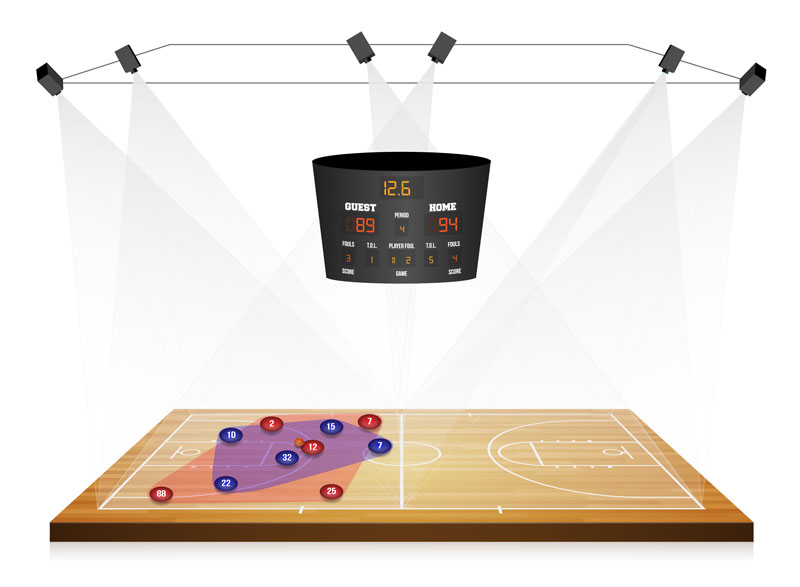
\includegraphics[width=0.6\textwidth]{images/sportVU}
    \caption{Diagrama informativo de la instalación de SportVU en un campo de baloncesto.}
    \label{fig:sportVU}
\end{figure}

Existen otras soluciones que permiten recabar estadísticas del partido, como es el caso de SportVU. El sistema, en el caso del fútbol, consiste en la colocación de 3 o 6 cámaras (en algunos sistemas más), y recaba datos tales como distancia viajada, velocidad media, velocidad máxima, mapas de calor, posesión, etc. Sin embargo, está disponible para más deportes, como baloncesto  (figura \ref{fig:sportVU}), fútbol americano, béisbol, hockey sobre hielo y rugby.

\begin{figure}
    \centering
    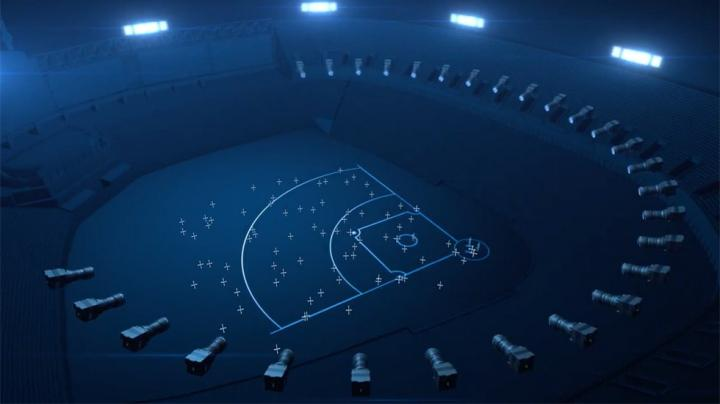
\includegraphics[width=0.6\textwidth]{images/intel360}
    \caption{Imagen promocional del sistema Intel 360 Replay.}
    \label{fig:intel360}
\end{figure}

Además podemos encontrar otros sistemas que se utilizan para análisis deportivo y/o ayuda al espectador de TV. Entre estos se encuentra el desarrollado por Intel: Intel 360 Replay (figura \ref{fig:intel360}). Este sistema ofrece repeticiones en 3D mediante el uso de 38 cámaras de resolución 5K. Se lleva usando durante unos años en la NBA y la MLB y recientemente en fútbol, siendo el clásico de la temporada pasada uno de los primeros grandes partidos en usarlo.

En deportes en los que el fondo es muy uniforme, como pueden ser los que emplean pistas de césped, se puede emplear para implementar un efecto de croma en la pista. Esto permite hacer dibujos en el campo de juego a fin de mostrar jugadas. También se ha empleado una técnica parecida durante la última fase de la temporada de LaLiga para sustituir las gradas vacías debido a la normativa sanitaria por imágenes de público.

Una de las áreas de investigación actuales es la de automatizar el control de cámaras durante las retransmisiones deportivas. Esta tarea es complicada ya que es un doble trabajo, requiere un seguimiento de la acción (que puede ser muy rápida por momentos) y la búsqueda de un buen plano que ayude al espectador a entender qué está pasando en el partido. Esta tecnología está aun muy lejos de ser una realidad en un futuro cercano. No obstante, un acercamiento es el de que un realizador controle una cámara principal, que es capaz de determinar de manera autónoma la posición a la que apunta, y una serie de cámaras ``esclavas'' apunten a dicha posición, de manera que se pueda ver la acción desde distintos puntos de vista \cite{book:cvInSports}.

Utilizando deep learning, se han publicado trabajos como el de \citet{art:DeepBall}, en el que se desarrolló un detector especializado en balones, utilizando una red completamente convolucional (figura \ref{fig:deepball}) y que produce un mapa de confianza con las posibles posiciones del balón. Este modelo era superior a otros dos anteriormente propuestos, logrando una precisión media de $87.7\%$, utilizando \textit{data augmentation}. Un problema que tenía el modelo eran las oclusiones de balón así como objetos de pequeño tamaño y de color similar al balón que engañaban al modelo (figura \ref{fig:deepballerror}).

\begin{figure}
    \centering
    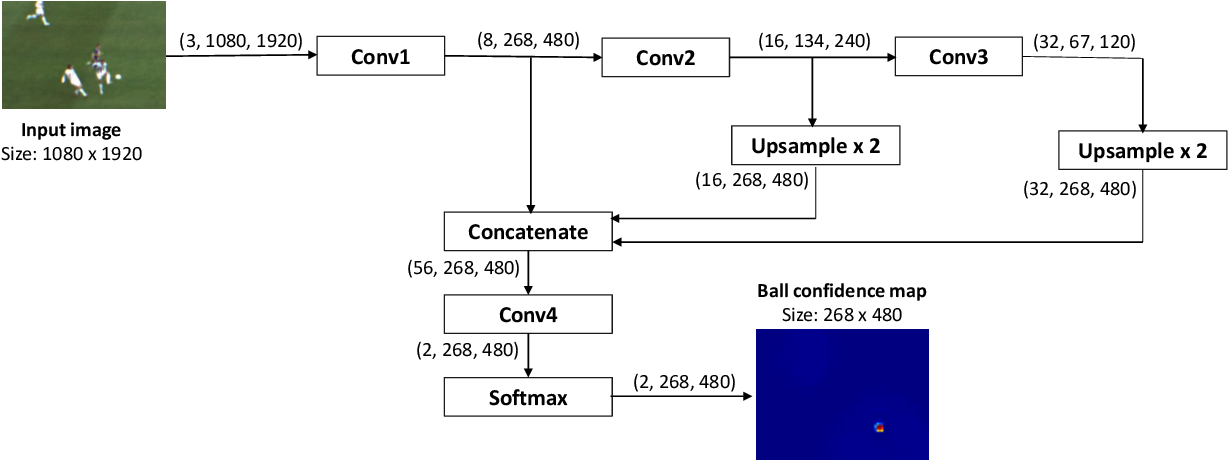
\includegraphics[width=0.7\textwidth]{images/deepball}
    \caption{Visualización de la arquitectura propuesta en DeepBall \cite{art:DeepBall}.}
    \label{fig:deepball}
\end{figure}


\begin{figure}
    \centering
    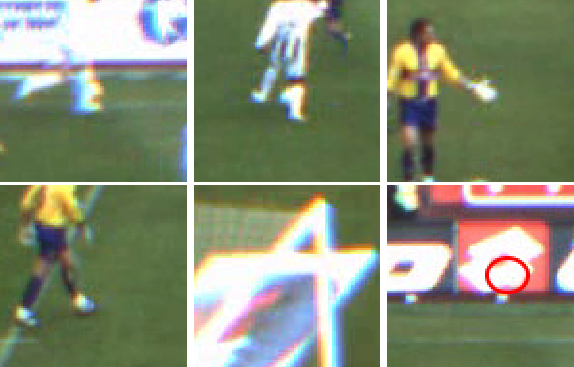
\includegraphics[width=0.4\textwidth]{images/errorDeepball.png}
    \caption{Algunos de los errores de detección del modelo DeepBall \cite{art:DeepBall}.}
    \label{fig:deepballerror}
\end{figure}

\newpage